% Created by tikzDevice version 0.12.6 on 2026-05-14 19:27:09
% !TEX encoding = UTF-8 Unicode
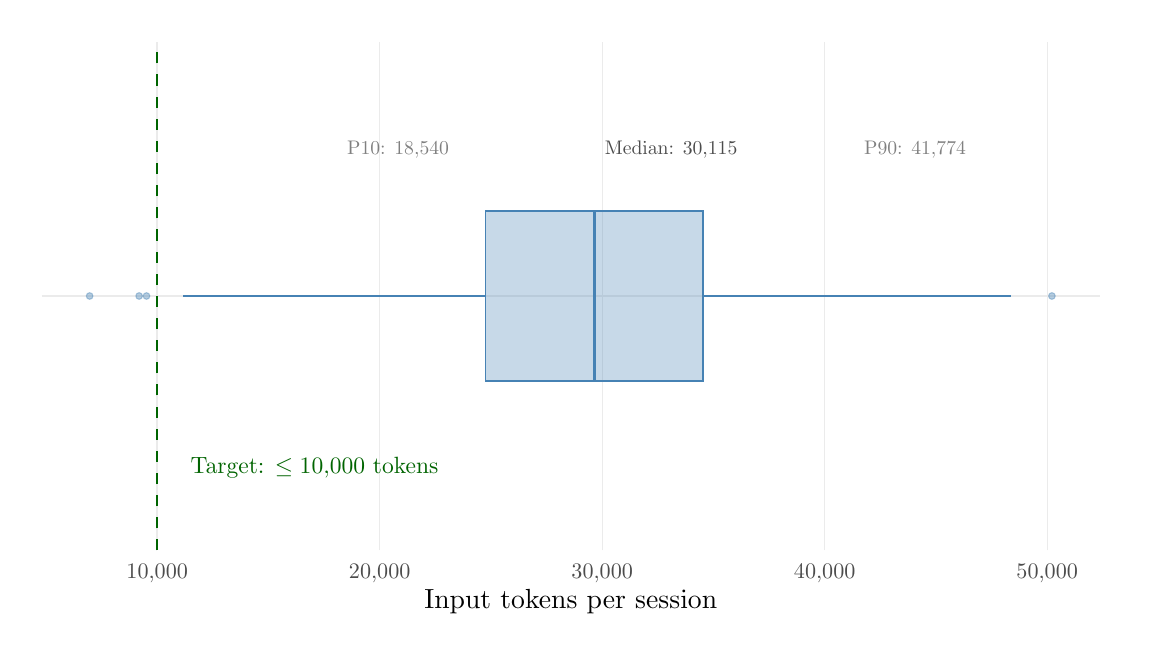
\begin{tikzpicture}[x=1pt,y=1pt]
\definecolor{fillColor}{RGB}{255,255,255}
\path[use as bounding box,fill=fillColor,fill opacity=0.00] (0,0) rectangle (397.48,216.81);
\begin{scope}
\path[clip] (  0.00,  0.00) rectangle (397.48,216.81);
\definecolor{fillColor}{RGB}{255,255,255}

\path[fill=fillColor] (  0.00,  0.00) rectangle (397.48,216.81);
\end{scope}
\begin{scope}
\path[clip] (  5.00, 27.90) rectangle (387.48,211.81);
\definecolor{drawColor}{gray}{0.92}

\path[draw=drawColor,line width= 0.5pt,line join=round] (  5.00,119.85) --
	(387.48,119.85);

\path[draw=drawColor,line width= 0.5pt,line join=round] ( 46.80, 27.90) --
	( 46.80,211.81);

\path[draw=drawColor,line width= 0.5pt,line join=round] (127.20, 27.90) --
	(127.20,211.81);

\path[draw=drawColor,line width= 0.5pt,line join=round] (207.60, 27.90) --
	(207.60,211.81);

\path[draw=drawColor,line width= 0.5pt,line join=round] (288.00, 27.90) --
	(288.00,211.81);

\path[draw=drawColor,line width= 0.5pt,line join=round] (368.40, 27.90) --
	(368.40,211.81);
\definecolor{drawColor}{RGB}{70,130,180}
\definecolor{fillColor}{RGB}{70,130,180}

\path[draw=drawColor,draw opacity=0.40,line width= 0.4pt,line join=round,line cap=round,fill=fillColor,fill opacity=0.40] ( 42.94,119.85) circle (  1.21);

\path[draw=drawColor,draw opacity=0.40,line width= 0.4pt,line join=round,line cap=round,fill=fillColor,fill opacity=0.40] ( 22.39,119.85) circle (  1.21);

\path[draw=drawColor,draw opacity=0.40,line width= 0.4pt,line join=round,line cap=round,fill=fillColor,fill opacity=0.40] (370.10,119.85) circle (  1.21);

\path[draw=drawColor,draw opacity=0.40,line width= 0.4pt,line join=round,line cap=round,fill=fillColor,fill opacity=0.40] ( 40.28,119.85) circle (  1.21);
\definecolor{drawColor}{RGB}{70,130,180}

\path[draw=drawColor,line width= 0.5pt,line join=round] (244.07,119.85) -- (355.31,119.85);

\path[draw=drawColor,line width= 0.5pt,line join=round] (165.51,119.85) -- ( 56.13,119.85);
\definecolor{fillColor}{RGB}{70,130,180}

\path[draw=drawColor,line width= 0.5pt,fill=fillColor,fill opacity=0.30] (244.07, 89.20) --
	(165.51, 89.20) --
	(165.51,150.51) --
	(244.07,150.51) --
	(244.07, 89.20) --
	cycle;

\path[draw=drawColor,line width= 1.0pt] (204.70, 89.20) -- (204.70,150.51);
\definecolor{drawColor}{RGB}{0,100,0}

\path[draw=drawColor,line width= 0.8pt,dash pattern=on 4pt off 4pt ,line join=round] ( 46.80, 27.90) -- ( 46.80,211.81);

\node[text=drawColor,anchor=base west,inner sep=0pt, outer sep=0pt, scale=  0.85] at ( 58.86, 55.61) {Target: $\leq 10{,}000$ tokens};
\definecolor{drawColor}{gray}{0.30}

\node[text=drawColor,anchor=base west,inner sep=0pt, outer sep=0pt, scale=  0.71] at (208.53,171.05) {Median: 30{,}115};
\definecolor{drawColor}{gray}{0.50}

\node[text=drawColor,anchor=base west,inner sep=0pt, outer sep=0pt, scale=  0.71] at (115.46,171.05) {P10: 18{,}540};

\node[text=drawColor,anchor=base west,inner sep=0pt, outer sep=0pt, scale=  0.71] at (302.26,171.05) {P90: 41{,}774};
\end{scope}
\begin{scope}
\path[clip] (  0.00,  0.00) rectangle (397.48,216.81);
\definecolor{drawColor}{gray}{0.30}

\node[text=drawColor,anchor=base,inner sep=0pt, outer sep=0pt, scale=  0.80] at ( 46.80, 17.89) {10,000};

\node[text=drawColor,anchor=base,inner sep=0pt, outer sep=0pt, scale=  0.80] at (127.20, 17.89) {20,000};

\node[text=drawColor,anchor=base,inner sep=0pt, outer sep=0pt, scale=  0.80] at (207.60, 17.89) {30,000};

\node[text=drawColor,anchor=base,inner sep=0pt, outer sep=0pt, scale=  0.80] at (288.00, 17.89) {40,000};

\node[text=drawColor,anchor=base,inner sep=0pt, outer sep=0pt, scale=  0.80] at (368.40, 17.89) {50,000};
\end{scope}
\begin{scope}
\path[clip] (  0.00,  0.00) rectangle (397.48,216.81);
\definecolor{drawColor}{RGB}{0,0,0}

\node[text=drawColor,anchor=base,inner sep=0pt, outer sep=0pt, scale=  1.00] at (196.24,  6.94) {Input tokens per session};
\end{scope}
\end{tikzpicture}
